\documentclass[../../main.tex]{subfiles}

\begin{document}

\section{Introduction}

In this paper, we examine tunnelling solutions to the 
fundamental equation in quantum mechanics: the Schr\"odinger equation
for a single particle.
\begin{equation}
		\label{eq:schrodinger}
		i \hbar \pder{\Psi}{t} = -\frac{\hbar^2}{2m} \nabla^2 \Psi + 
		V \Psi
\end{equation}
Here $\Psi = \Psi(\vec x)$ is the wave function describing a 
quantum mechanical particle, $t$ is time, 
$V = V(\vec x, t)$ is the potential with which the particle 
interacts.  The constant $m$ is the mass of the particle,
and $\hbar$ is Planck's constant divided by $2\pi$ 
\cite{griffiths-quantum}.  

We consider the following scenario. 
A particle is confined to a well in $\R^2$.  
It passes by a ring-shaped well which is connected to a 
second well leaving the system
(see figure \ref{fig:system-sketch}).
Such a situation is the problem of interest in characterizing
quantum ring resonators \textbf{TODO: citation}.

\begin{figure}[h]
		\centering
		\includegraphics[width=0.5\textwidth]{system-sketch.png}
		\caption{Sketch of Ring resonator. 
		The domain excluding the shaded regions is $\Omega_0$. 
		The two shaded rectangles are $\Omega_1$ and $\Omega_2$ from
		left to right.  Finally the center ring is 
		$\Omega_3$.  
		The entire domain is $\Omega = \Omega_0 \cup \Omega_1 \cup 
		\Omega_2 \cup \Omega_3.$}
		\label{fig:system-sketch}
\end{figure}

We will solve this problem using finite elements, and using 
the Python library FEniCS, which will take care of the heavy lifiting
in constructing the finite element representation, as well as solving
the resulting linear algebra system.

Let $\Omega_0$ be the region without color, a rectangle of width 
$W$ and length $L$, excluding the colored regions.
The two long rectangles, in order from left to right are $\Omega_1$ and 
$\Omega_2$ respectively.  Finally, the ring in the center is 
$\Omega_3$.



\subsection{Nondimensionalization}

Nondimensionalizing the problem is essential since 
$\hbar \approx 10^{-34} J \cdot s$ in S.I. units.  
Let the spacial scaling be $d$, the width of each of the long potential 
wells.  
This induces a time scaling of 
$\frac{2m d^2}{\hbar}$.  
Finally there is an energy scaling of $V_0$, which characterizes the 
strength of the potential.
To summarize, 
if $\tilde{\vec x}, \tilde t, \tilde V$ all have units, then
\begin{equation}
		\label{eq:nd}
		\tilde{\vec x} = d \cdot \vec x, \quad 
		\tilde t = \frac{2m d^2}{\hbar} t, \quad 
		\tilde V(\tilde{\vec x}) = V_0 V(\vec x)
.\end{equation}
Let $\nu = \frac{2md^2 V_0}{\hbar^2}$.  
The nondimensionalized problem then reads
\begin{equation}
		\label{eq:schrodinger-nondim}
		i \pder{\Psi}{t} = -\nabla^2 \Psi + \nu V(\vec x) \Psi
.\end{equation}
Here, the form of $V(\vec x)$ is 
\begin{equation}
		\label{eq:potential-nondim}
		V(\vec x) = 
		\begin{cases}
				-1 & \vec x \in \Omega_1 \cup \Omega_2 \cup \Omega_3 \\
				0 & \vec x \in \Omega_0
		\end{cases}
.\end{equation}

\subsection{Boundary and Initial Conditions}

An input is specified on the lower portion of the left-most 
shaded rectangle.  
This will be denoted by the region $\Gamma_\mathrm{in}$.  
All other boundaries of $\Omega$ which are also boundaries of 
$\Omega_i$ for $i = 1, 2$ will be denoted 
$\Gamma_\mathrm{out}$.  
Finally, the rest of the boundary will be denonted $\Gamma_D$.  

On $\Gamma_\mathrm{in}$, there is a specified Dirichlet boundary condition:
$f(\vec x, t)$, and on $\Gamma_D$ the Dirichlet condition is zero.
Lastly, on $\Gamma_\mathrm{out}$ we specify an outflow boundary condition.
In quantum mechanics, the momentum operator, 
in this dimensionless system: $\hat{\vec p} = -\frac{i \hbar}{d} \nabla$.
The outflow condition relates $\partial_t \psi$ with the momentum. 
All together the boundary conditions are
\begin{equation}
		\label{eq:boundary-conditions}
		\text{Boundary Conditions} = 
		\begin{cases}
				\Psi(\vec x, t) = 0 & \vec x \in \Gamma_D \\
				\Psi(\vec x, t) = f(\vec x, t) & \vec x \in \Gamma_\mathrm{in}
				\\
				\pder{\Psi}{t} = -2i  \pder{\Psi}{n} & 
				\vec x \in \Gamma_\mathrm{out}
		\end{cases}
\end{equation}
Where $f(\vec x, t)$ is a prespecified function.

Finally for simplicity, we take an initial condition of 
an empty system: i.e.
\[
		\Psi(\vec x, 0) = 0
.\] 
\end{document}
